% THIS IS SIGPROC-SP.TEX - VERSION 3.1
% WORKS WITH V3.2SP OF ACM_PROC_ARTICLE-SP.CLS
% APRIL 2009
%
% It is an example file showing how to use the 'acm_proc_article-sp.cls' V3.2SP
% LaTeX2e document class file for Conference Proceedings submissions.
% ----------------------------------------------------------------------------------------------------------------
% This .tex file (and associated .cls V3.2SP) *DOES NOT* produce:
%       1) The Permission Statement
%       2) The Conference (location) Info information
%       3) The Copyright Line with ACM data
%       4) Page numbering
% ---------------------------------------------------------------------------------------------------------------
% It is an example which *does* use the .bib file (from which the .bbl file
% is produced).
% REMEMBER HOWEVER: After having produced the .bbl file,
% and prior to final submission,
% you need to 'insert'  your .bbl file into your source .tex file so as to provide
% ONE 'self-contained' source file.
%
% Questions regarding SIGS should be sent to
% Adrienne Griscti ---> griscti@acm.org
%
% Questions/suggestions regarding the guidelines, .tex and .cls files, etc. to
% Gerald Murray ---> murray@hq.acm.org
%
% For tracking purposes - this is V3.1SP - APRIL 2009

\documentclass{acm_proc_article-sp}

\begin{document}

\title{Assignment B}
\subtitle{02806 Social data analysis and visualization}

\numberofauthors{1}
\author{
% 1st. author
\alignauthor
Anders Hørsted\\
       \affaddr{s082382}\\
       \email{anders@dinero.dk}
}

\date{12 May 2014}

\maketitle

\begin{figure}
    \centering
    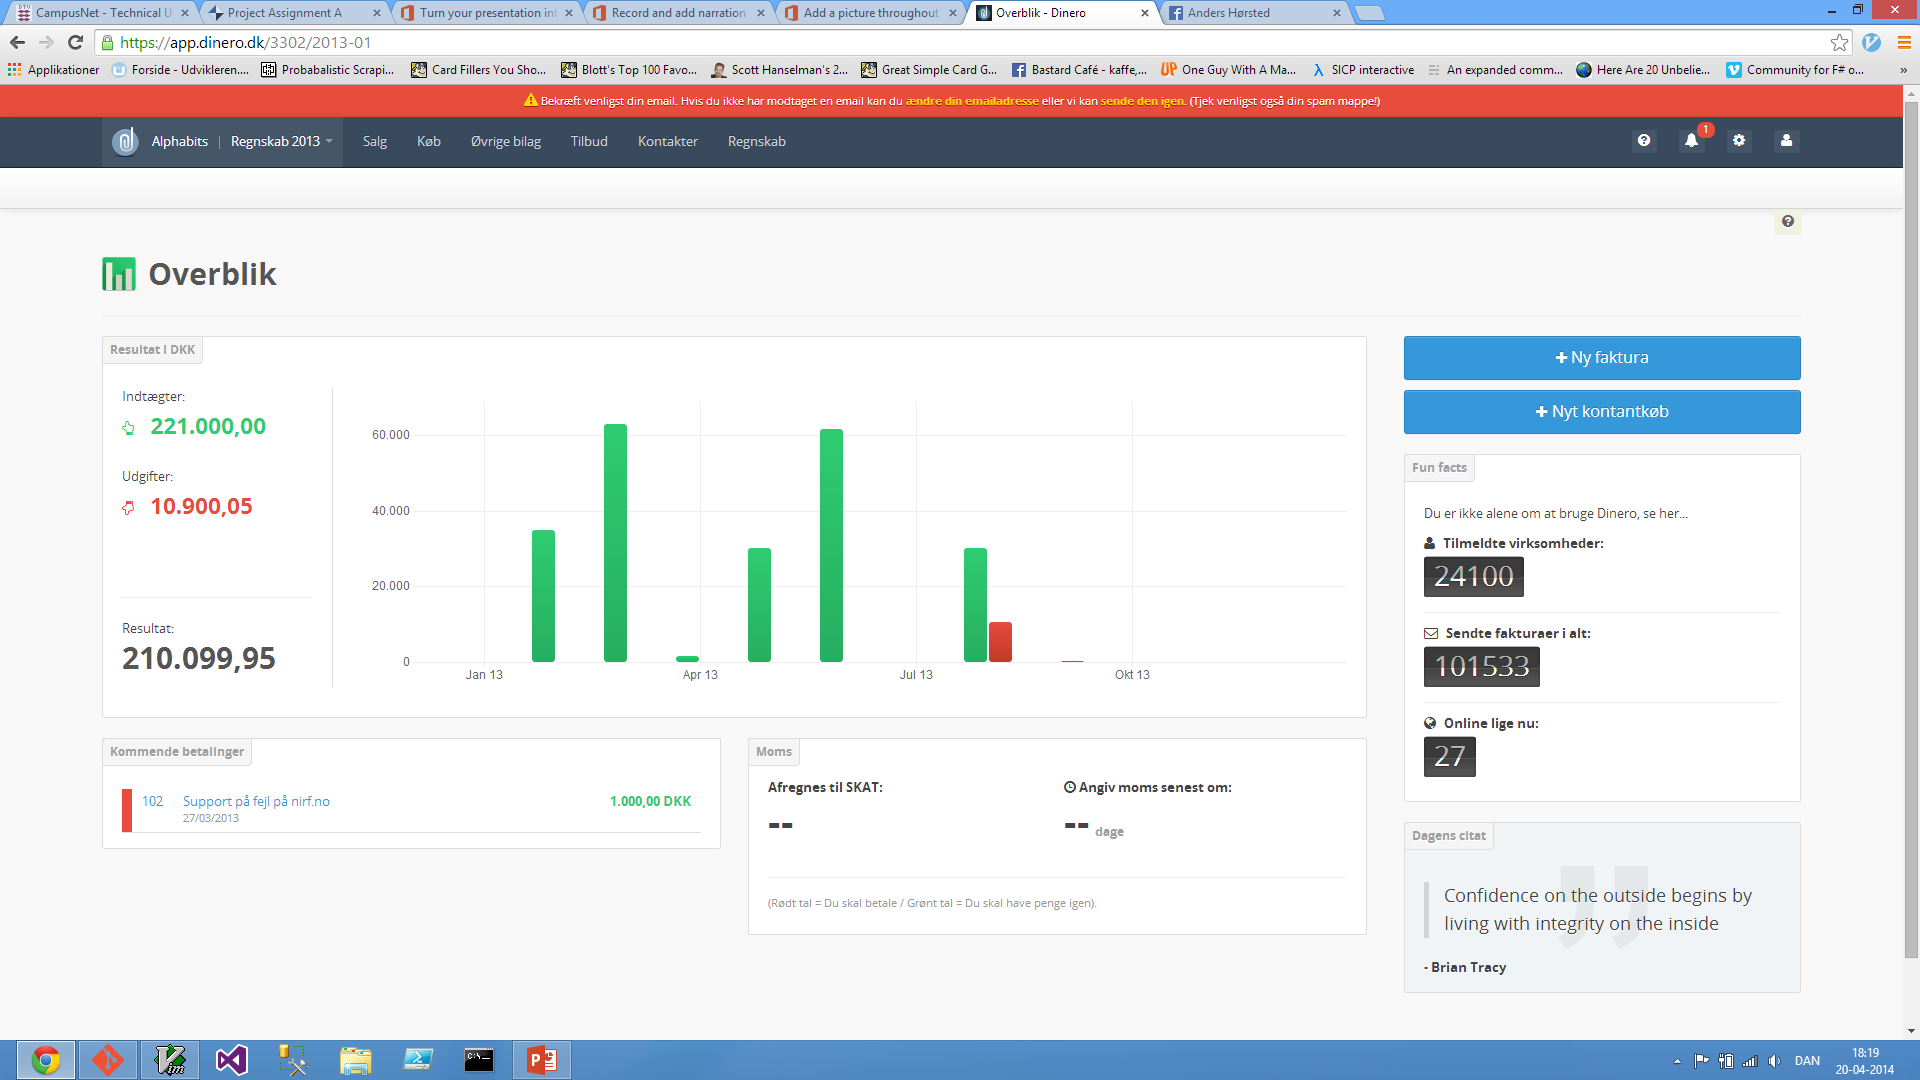
\includegraphics[width=\columnwidth]{dinero-home-screenshot.png}
    \caption{The start page when logged in to Dinero}
    \label{fig:homepage}
\end{figure}

\section{Motivation}
In this section the dataset analyzed in this assignment is introduced and the reasons for choosing this specific dataset is given.

The dataset that needs to be analyzed is data from the main database of the danish online accounting application www.dinero.dk. Dinero has been public since April 2013 and so far more than 25.000 users have signed up. Dinero is using a classic Freemium\footnote{http://en.wikipedia.org/wiki/Freemium} pricing strategy where the basic application is free for use. To entice free users to upgrade to become paying pro users various features (eg. upload pictures of vouchers to the cloud) are only available for pro (paying) users. Since the lauch in April 2013 and until now all work has been focused on developing new features for the application and fixing bugs in the existing codebase, but now it is time to get some insights into the userbase of Dinero. How many users are actually using the application? How many vouchers are created every day? And how many users are upgrading from free to pro user?

To answer these questions a simple dashboard (see figure~\ref{fig:dashboard}) is created and some basic analysis of the graphs of the dashboard is performed. The motivation to do this work is that various stakeholders of Dinero are eager to get better insight into the usage of Dinero. 

The final dashboard is created within the codebase of the public dinero application and is found at the url 

\textbf{http://app.dinero.dk/showmesomenumbers}

Please keep this url secret since the dashboard isn't intended to be public available and will be password protected as soon this assignment has been evaluated. 
%Also note that the dashboard will be available from May 13 since it needs to be published along with the usual deployment schedule used in Dinero.

\subsection{Introduction to various Dinero concepts}

To better understand the Dinero dashboard a few central concepts in Dinero are mentioned in this section. A human being that signup to Dinero is called a \textbf{User}. A User can create one ore more \textbf{Organization}s. If a User want to use some of the advanced features for a Organization he has to buy a pro \textbf{Subscription} for the Organization. One of the most important objects a User creates within an Organization is \textbf{Voucher}s (danish: bilag).

\begin{figure}
    \centering
    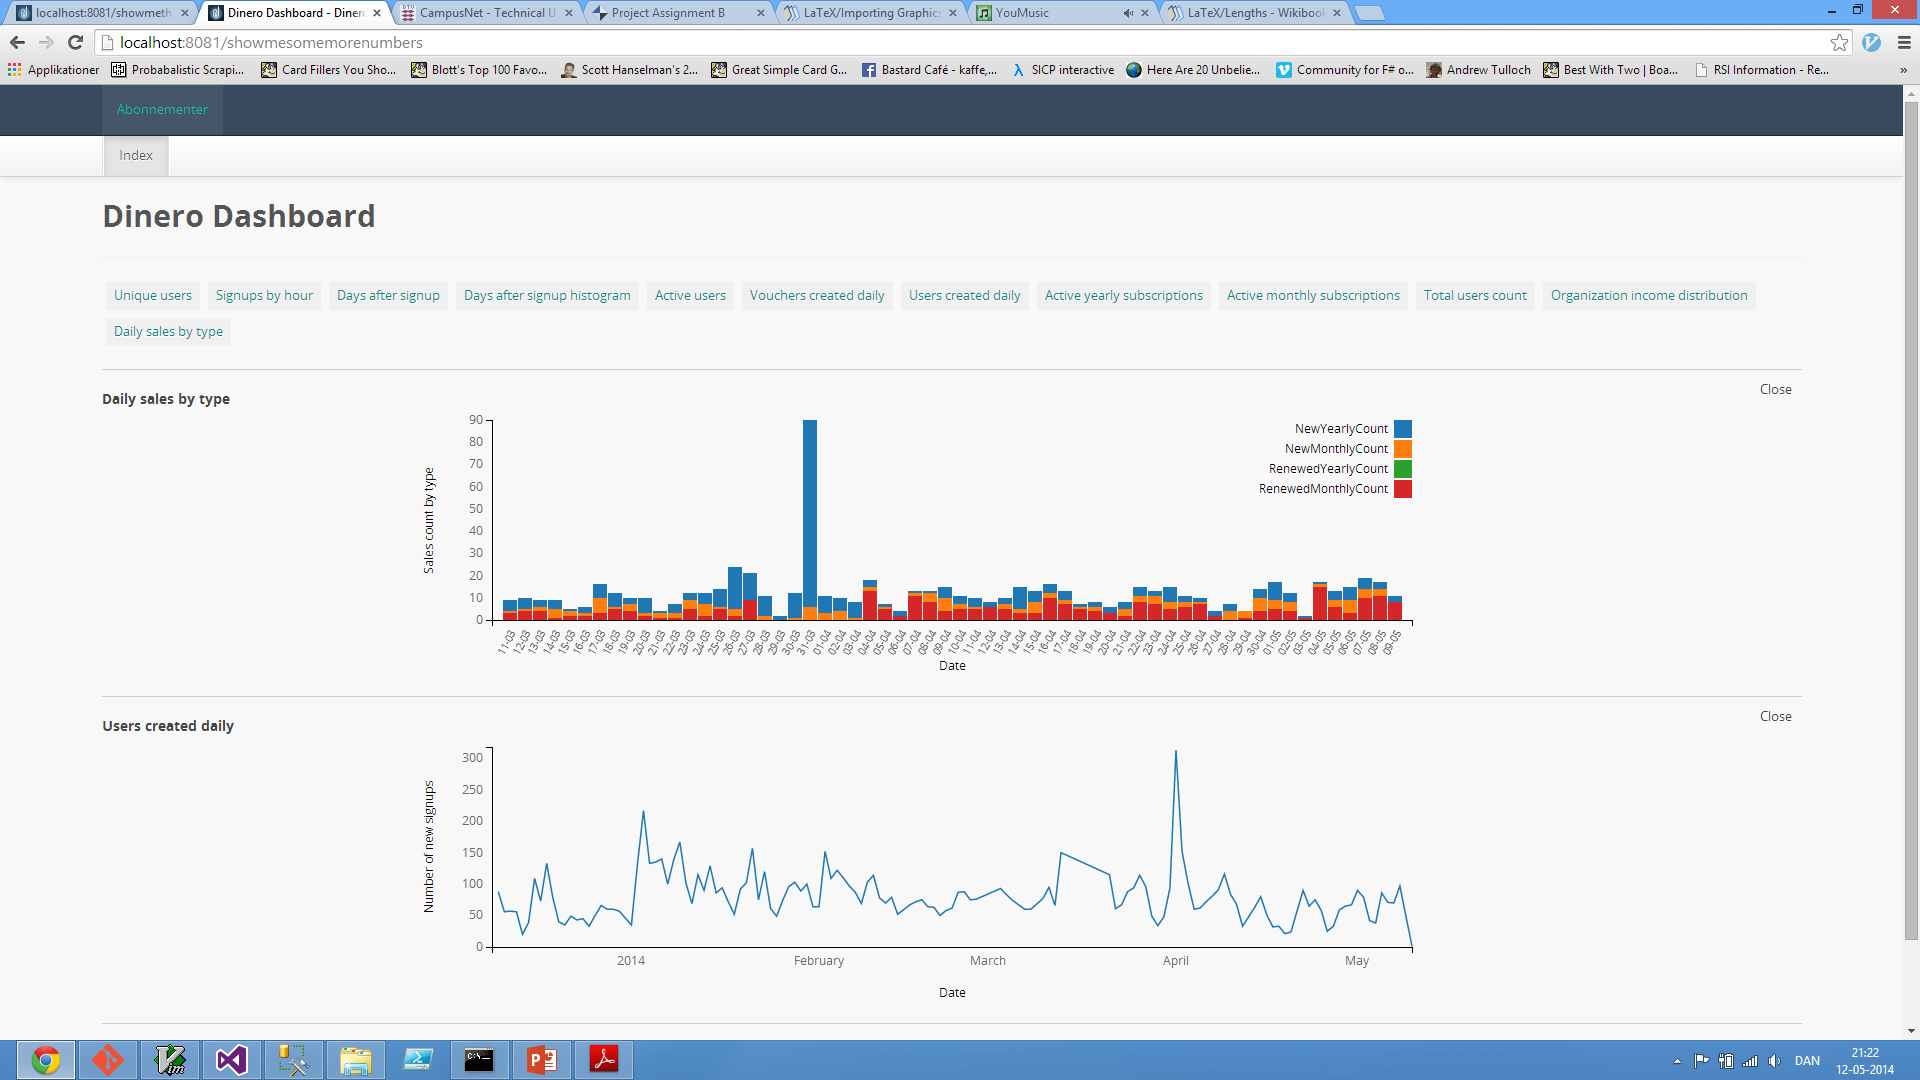
\includegraphics[width=\columnwidth]{dinero-dashboard.png}
    \caption{The dashboard developed for Dinero}
    \label{fig:dashboard}
\end{figure}

%What is your dataset? Why did you choose that one? What is your goal for the end user's experience?


\section{Theory}

In this section the theory used is introduced and the various graphs of the dashboard are described. Due to many technical problems (see Discussion) some of the more interesting analysis techniques (eg. decision tree to classify users into groups) haven't been used in the dashboard and all graphs are just various visualizations of data in the Dinero database.

\subsection{Analysis}

In this section a few of the graphs from the dashboard are analysed.

\subsubsection{Sales count by type}

This graph is shown in figure~\ref{fig:daily-sales} and is a stacked bar chart where the sales count for 4 different categories are shown for the past 50 days. The 4 categories are New Yearly Subscription, New Monthly Subscriptions, Renewed Yearly Subscriptions and Renewed Yearly Subscriptions. From the graph it is seen that there is quite some variation between days with many new subscriptions and days with primarily renewals. Also it is seen that the 31 March 2014 is a special day with over 90 sales.

\begin{figure}
    \centering
    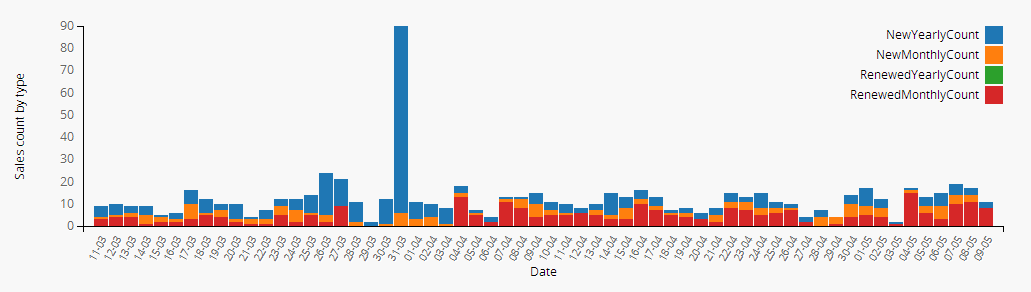
\includegraphics[width=\columnwidth]{sales-count-by-type.png}
    \caption{The daily sales grouped by type}
    \label{fig:daily-sales}
\end{figure}

\subsubsection{Number of days between signup and first pro subscription}

The graph is shown in figure~\ref{fig:days-after-signup} and shows a histogram of the number of days from a user signs up until he becomes a paying pro user. This graph is very interesting since the number of days a user needs to use the free until he is convinced that Dinero is worth the money is a good measure for the potential of Dinero to become a commercial success. And the results are actually very encouraging. Out of some 800 pro users 190 users bought a pro subscription within the first 20 days after signup. 90 users needed between 20-40 days and the rest needed more than 40 days. This was better than expected.

\begin{figure}
    \centering
    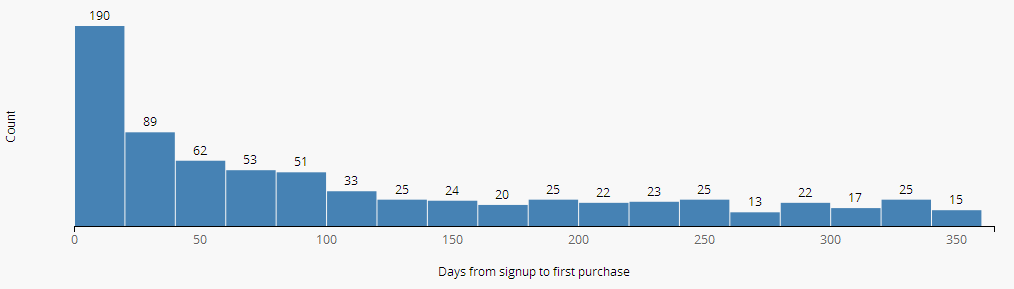
\includegraphics[width=\columnwidth]{days-after-signup-histogram.png}
    \caption{Histogram for the number of days from signup until first payment}
    \label{fig:days-after-signup}
\end{figure}


\subsubsection{Income distribution for organizations}

In figure~\ref{fig:organization-income} is shown a histogram of the distibution of income for the approx. 10000 organizations that have registered an income between 0 and 1200000 DKK and who do not have a pro subscription at the moment. This is of interest since all organization with an income above 1000000 DKK are forced to upgrade to a pro account. Organizations with an income close to 1000000 DKK is therefore likely to become paying customers in the near future. From the graph it is seen that the majority of all organizations have incomes below 500000 DKK and that we should only expect to upgrade maybe 60 organizations in the near future.

\begin{figure}
    \centering
    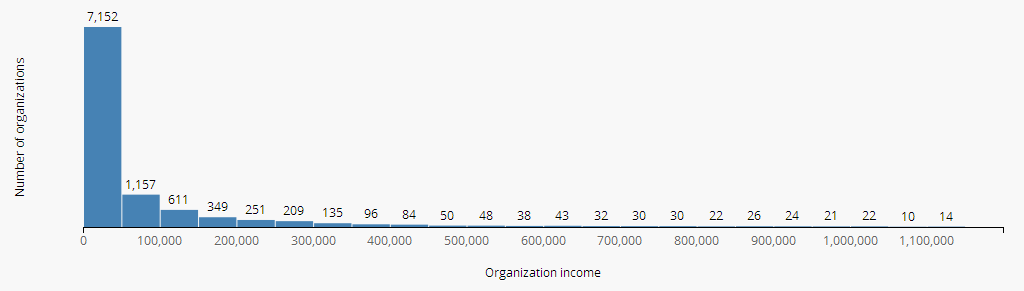
\includegraphics[width=\columnwidth]{income.png}
    \caption{Histogram for organization income}
    \label{fig:organization-income}
\end{figure}

\section{Implementation}

In this section the tools used to create the dashboard are described. The dashboard was created within the main Dinero web application. The Dinero application is an ASP.Net MVC application that communicates with a restful api created with ASP.Net WebApi. The dashboard is a single webpage where most of the content is generated by Javascript. To structure the Javascript code Backbone.js\footnote{http://backbonejs.org} was used and to create all graphs the D3-library\footnote{http://d3js.org} was used. To get the data for the graphs various SQL-Queries was created and to send the data to the browser some new Api-endpoint was created in the Dinero Api.

%How did you go about implementing your idea? Which practical tools did you use?

\section{Discussion}

As already mentioned in the Theory section the interesting analysis teckniques haven't been used in this assignment. From the outset it was planned to create a dynamic dashboard including a decision tree that could classify users most likely to become paying customers. If time permitted it was also the plan to do some sentiment analysis of our facebook and twitter messages. Unfortunately the time needed to just get some usable data out of the Dinero database and create even simple graphs with the D3-library was greatly underestimated. In retrospect a library on top of D3 should probably have been used, and much more time allocated to get useful data out of the database. 

On the positive side a knowledge of the inner workings of the D3 library have been obtained and the dashboard have received very positive feedback from some of Dinero stakeholders (not including the author of this paper).

\balancecolumns
\end{document}  % This is where a 'short' article might terminate

%
% The following two commands are all you need in the
% initial runs of your .tex file to
% produce the bibliography for the citations in your paper.
%\bibliographystyle{abbrv}
%\bibliography{sigproc}  % sigproc.bib is the name of the Bibliography in this case
% You must have a proper ".bib" file
%  and remember to run:
% latex bibtex latex latex
% to resolve all references
%
% ACM needs 'a single self-contained file'!
%
%APPENDICES are optional
%\balancecolumns
%\appendix
%Appendix A
% That's all folks!
%\end{document}
